\section{Optimizing t-SNE}

\begin{frame}{Initialization}
    \begin{itemize}
        \item It is best to use "informative initialization" instead of random initialization for t-SNE. 
        \item PCA initialization better preserves global structure.  
    \end{itemize}
    \begin{figure}
        \centering
        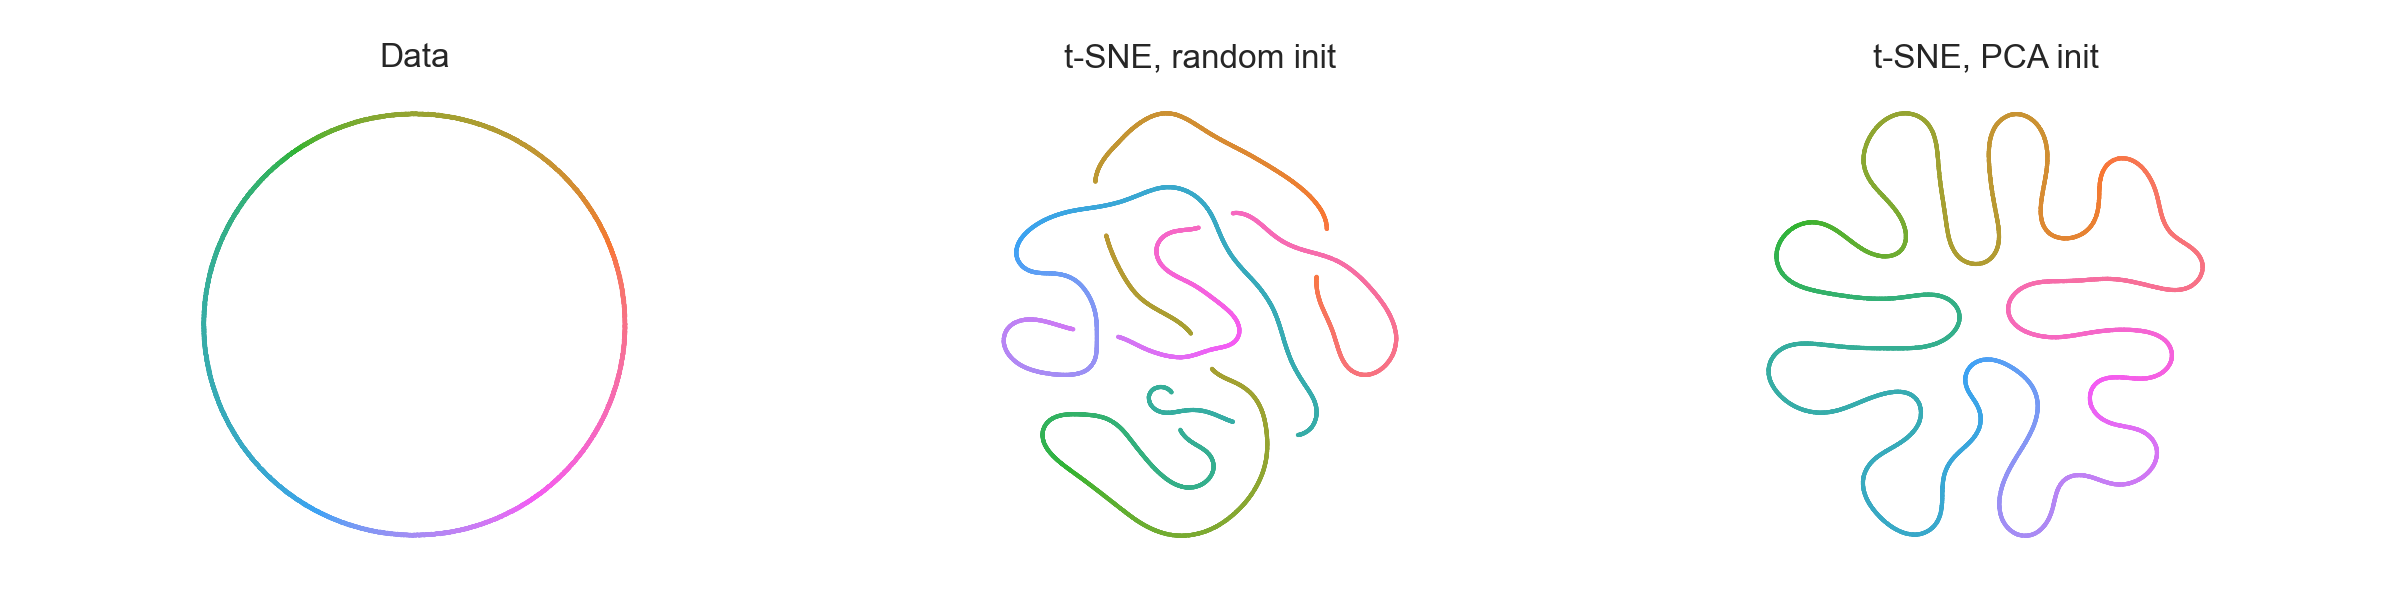
\includegraphics[width=\textwidth]{tsne-circle.png}
        \caption{The t-SNE algorithm only produces a faithful representation of the circle with informative initialization. Visualization reproduced from \cite{kl2021}}. 
    \end{figure} 
\end{frame}

\begin{frame}{Perplexity}
    \begin{itemize}
        \item Recall \[p_{i|j} = \frac{\exp(-||x_i-x_j||^2/2\sigma_i^2)}{\sum_{k\neq i} \exp (- ||x_i - x_k||^2/2\sigma_i^2)}.\] How do we choose the bandwidth $\sigma_i$ of the Gaussian kernel centered at $x_i$? \pause
        \item It depends on the data! In dense regions, we want a smaller $\sigma_i$ than in sparse ones.  \pause 
    \end{itemize}
    \begin{definition}[Shannon Entropy]
        Let $X$ be a discrete random variable taking values in $\mathcal{X}$ which is distributed according to $p: \mathcal{X} \to [0,1]$, then the Shannon Entropy is $H(X) = - \sum_{x \in \mathcal{X}} p(x) \log_2 (p(x))$.
    \end{definition}
    \begin{itemize}
        \item We define a constant \textbf{perplexity} value 
        \[ \text{Perp}(P_i) = 2^{H(P_i)} = 2^{-\sum_{j} p_{j|i} \log p_{j|i}}\] where $P_i$ is the probability distribution induced by $\sigma_i$. \pause
        \item Perplexity effectively measures the number of neighbours we wish to consider.  
    \end{itemize}
\end{frame}

\begin{frame}{Perplexity}
    \begin{figure}
        \centering
        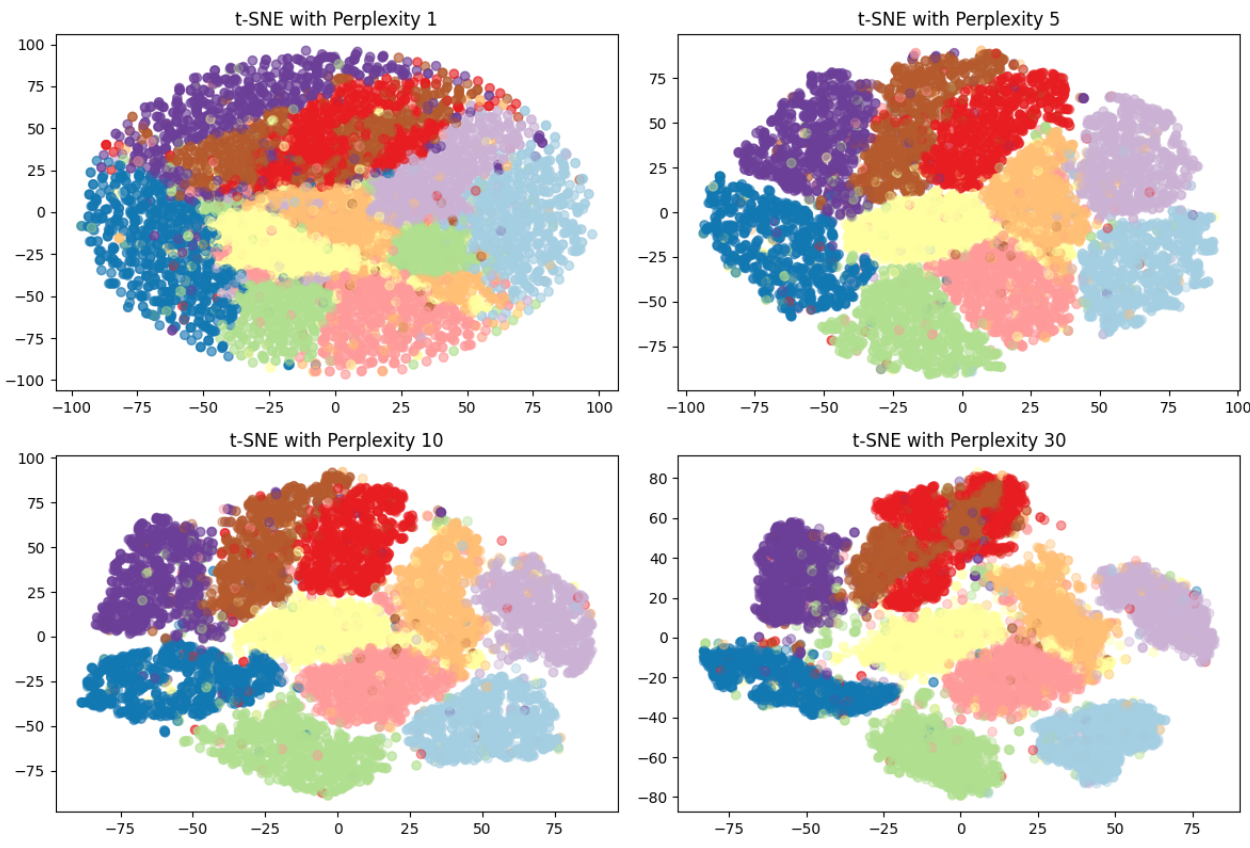
\includegraphics[width=0.8\textwidth]{varying_perplexity.png}
        \caption{Different perplexity values on the MNIST dataset.}
    \end{figure} 
\end{frame}

\begin{frame}{Perplexity}
    \begin{figure}
        \centering
        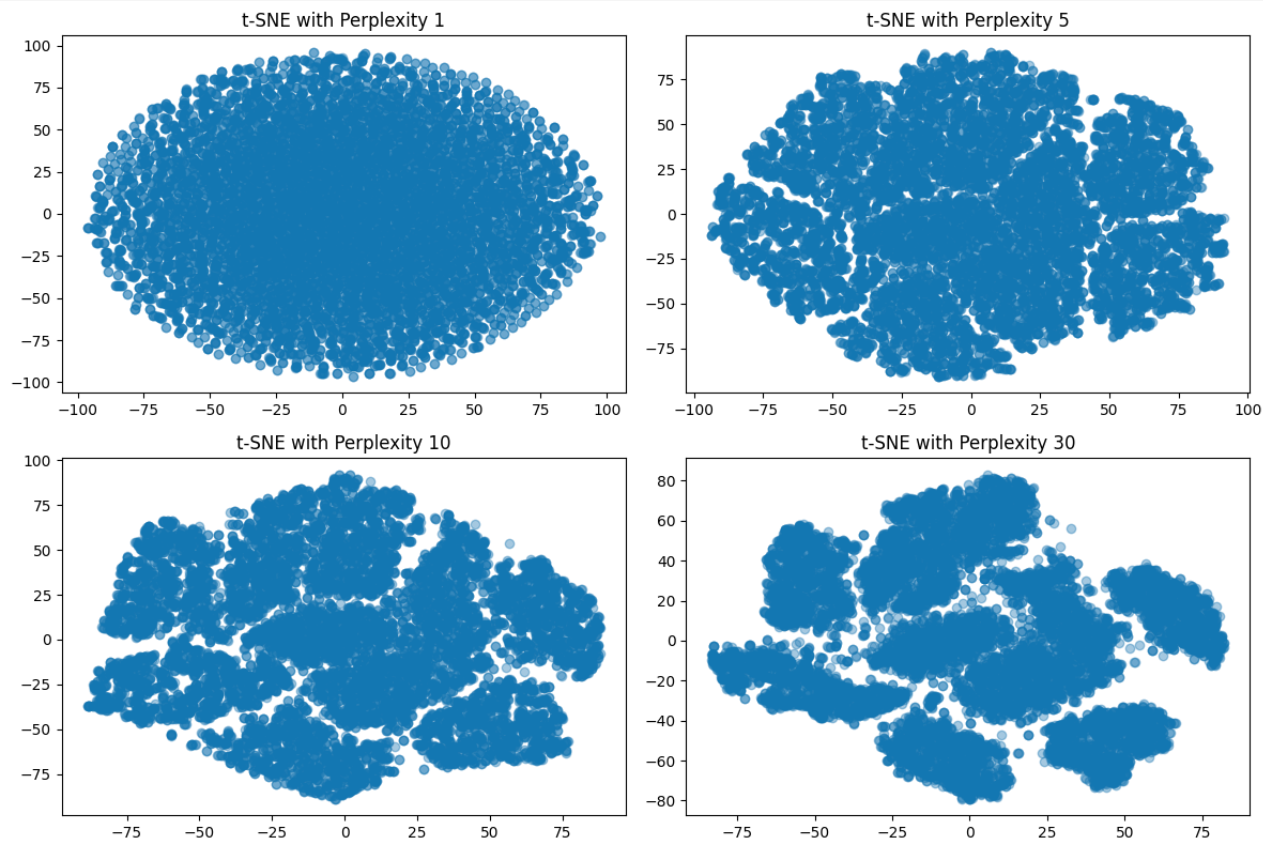
\includegraphics[width=0.83\textwidth]{perplexity_without_gt.png}
        \caption{Different perplexity values on the MNIST dataset without ground truth labels.}
    \end{figure} 
\end{frame}

\begin{frame}{Early Exaggeration}
    \begin{itemize}
        \item \textbf{Idea}: in early iterations of t-SNE we want to focus on tight cluster formation and only worry about "nice" visualization later on \pause
        \item We multiply all $p_{ij}$ by a certain factor $\alpha$ (standard value is $\alpha= 12$) for the first few iterations (standard: $250$). 
        \item Clusters can more easily move around in space later on. \pause 
        \item In the attraction-repulsion framework: 
        \[ \frac{1}{4} \frac{\partial C}{\partial y_i} = \sum_{i\neq j} \alpha p_{ij} q_{ij} Z (y_i - y_j) - \sum_{j \neq i} q_{ij}^2 Z (y_i - y_j)
        \] \pause 
        \item \textbf{Question}: How do we find good values for $\alpha$ and for how many iterations should we keep early exaggeration on? 
    \end{itemize}
\end{frame}

\begin{frame}{Automated Optimized Parameters}
    \begin{figure}
        \centering
        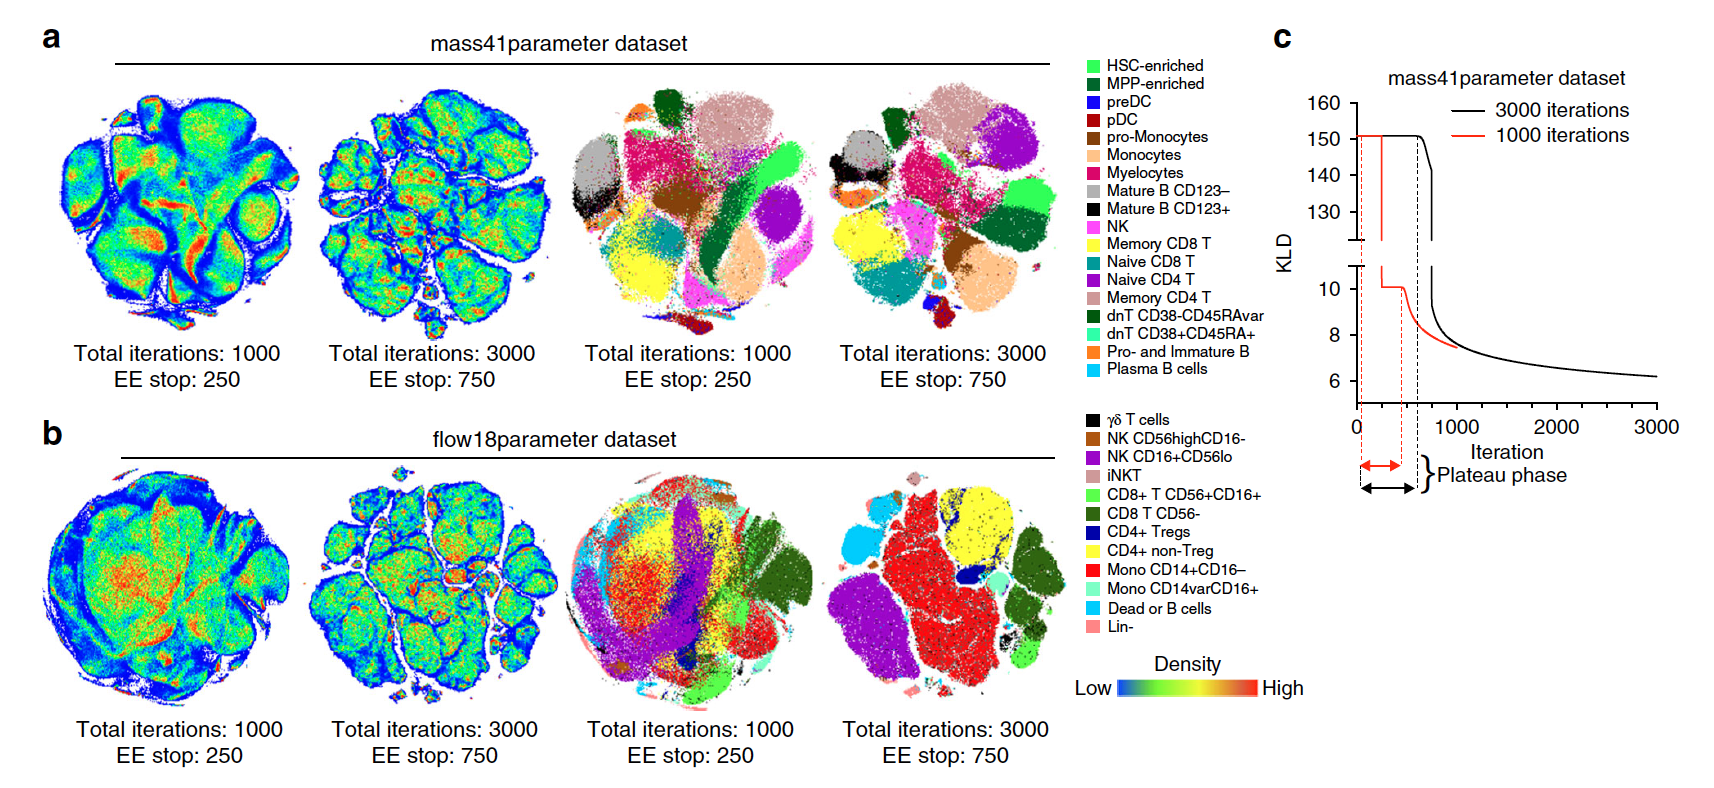
\includegraphics[width=\textwidth]{nature_EE_stop.png}
        \caption{Performance of t-SNE for cytometry data visualization, see \cite{belkina2019}.}
    \end{figure} 
\end{frame}

